\subsection{Neural Networks Test}
The main functionality of my library, is to allow users to create a convolutional or a dense neural network. Therefore, it is important that I test this functionality out and make sure it works correctly. This test, unlike the previous tests, is an integration test as I will be testing out many classes at the same time, including the Volume, Matrix, Net, Conv, Dense, MaxPool, Reshape, Mapping, Optimiser and netData classes. Therefore, by doing this integration test I will also know how well the constituent parts of my project work together.
\\
It would be incredibly difficult to test whether a neural network works and whether the back propagation algorithm works by tracing each step. However, I can still test whether the network learns from the data given by comparing how well it performs against the data and how each back-propagation algorithm allows the network to learn. It is important to note that the conv-layers are used in conjunction with the Dense layer, therefore it is first necessary to test whether the dense layers work before moving on to the conv-layers.
\\ \\
I will now be testing the dense layers, using the squared error as my loss function and using 500 training iterations.
The training data that I will be using will be $x = matrix.join(x_1, x_2)$, where $x_1 \sim N(3, 1)$ \& $x_1.shape = (5, 50)$ and $x_1 \sim N(0, 2)$ \& $x_2.shape = (5, 50)$.
\\
This means, that I will be having a data-set of 100 examples with 5 features and the network will try to distinguish between the two data-sets. If the data belongs in $x_1$, then the net will need to predict a 1 else it needs to predict a 0.
\\
To see if the net has learnt the data, I will be testing it with a test set which will have the same shape as $x$, but the difference being that it will have different values. In these tests the Net should learn the function to an appropriate degree of accuracy with all hyper parameters kept constant besides the mini-batch size and learning rate. In these tests the Net should achieve at least a minimum loss of 0.01 for a test to be said to be successful. 
\\
I will be recording the average loss for a particular test using 100 different tests for the same architecture and optimiser.
\\ \\
The following table below shows the results of the test. The net architecture describes the number of layers in each net and the activation used.

\begin{table}[H]
\centering
    \begin{tabular}{|p{1cm}|p{5cm}|p{2cm}|p{2cm}|}
        \hline
        Test No. & Net Architecture & Optimiser & Final loss\\ \cline{1-4} 
        1.0 & 4-relu, 3-relu, 1-sigmoid & GDO & 0.0099\\ \cline{1-4}
        1.1 & 4-relu, 3-relu, 1-sigmoid & ADAM & 0 \\ \cline{1-4}
        1.2 & 4-relu, 3-relu, 1-sigmoid & Mom & 0.0031 \\ \cline{1-4}
        1.3 & 4-relu, 3-relu, 1-sigmoid & RMS & 0.0023 \\ \cline{1-4}
        
        2.0 & 4-tanh, 2-swish, 2-sigmoid, 1-sigmoid & GDO & 0.003 \\ \cline{1-4}
        2.1 & 4-tanh, 2-swish, 2-sigmoid, 1-sigmoid & ADAM & 0 \\ \cline{1-4}
        2.2 & 4-tanh, 2-swish, 2-sigmoid, 1-sigmoid & MOM & 0.007 \\ \cline{1-4}
        2.3 & 4-tanh, 2-swish, 2-sigmoid, 1-sigmoid & RMS & 0.001 \\ \cline{1-4}
        
        3.0 & 5-tanh, 3-relu, 1-sigmoid & GDO & 0.0054 \\ \cline{1-4}
        3.1 & 5-tanh, 3-relu, 1-sigmoid & ADAM & 0.0019 \\ \cline{1-4}
        3.2 & 5-tanh, 3-relu, 1-sigmoid & MOM & 0.0007 \\ \cline{1-4}
        3.3 & 5-tanh, 3-relu, 1-sigmoid & RMS & 0.0008 \\ \cline{1-4}
        
        4.0 & 7-swish, 1-sigmoid & GDO & 0.0002 \\ \cline{1-4}
        4.1 & 7-swish, 1-sigmoid & ADAM & 0.0001 \\ \cline{1-4}
        4.2 & 7-swish, 1-sigmoid & MOM & 0.0007 \\ \cline{1-4}
        4.3 & 7-swish, 1-sigmoid & RMS & 0 \\ \cline{1-4}
        
        5.0 & 1-sigmoid & GDO & 0.0099 \\ \cline{1-4}
        5.1 & 1-sigmoid & ADAM & 0.0001 \\ \cline{1-4}
        5.2 & 1-sigmoid & MOM & 0.0015 \\ \cline{1-4}
        5.3 & 1-sigmoid & RMS & 0.0011 \\ \cline{1-4}
    \end{tabular}
    \caption{Dense Neural Network Test}
\end{table}
From this table, we can see that the gradient descent optimises are working as they should and that the net is calculating the gradients correctly. This integration test shows that the constituent parts are functioning together correctly as no exceptions turned up, which shows that the algorithms have been implemented carefully as no overflow occurred. Furthermore, the time taken for this test was 2 hours as each test was repeated 100x. Finally, this test was again repeated 8x using different training sets, but the results were all successful.
\\
The conv layers, unlike the dense layers, do not have these advanced optimisation methods, therefore, I will only need to test out the gradient descent optimiser(GDO), for the conv layers. One important point to note is that training the conv layers can take a long time, possibly around 6 hours, depending upon the size of the data if the tests are to be repeated many times to obtain reliable results.

The data-set I will be using for the conv layers will be the MNIST data set, which consist of a data-set of hand-written digits. This data-set has been collected for the purpose of machine learning, therefore by using this data-set I will be able to achieve reliable results.

The notation being used to represent the net architecture is:
\begin{itemize}
    \item $c=(f, k_x, k_y, s_x, s_y)_a$ will denote a convolutional layer, with kernel of dimension $(k_x, k_y, f)$ with strides of $(s_x, s_y)$, activation $a$ and padding set to the default value: "valid".
    The activations that will be used are relu(r), sigmoid(s) and swish(sw)
    \item $m=(k_x, k_y, s_x, s_y)$ will denote a max-pooling layer, with kernel of dimension $(k_x, k_y)$ with strides of $(s_x, s_y)$ and activation $a$.
\end{itemize}
The notation to represent the dense nets that follow on after the conv nets will use the same notation as before. Finally, the softmax function will be used at the end to make a prediction for a specific class, and the loss function that will be used will be the softmax cross entropy cost function.
Due to the limited amount of time and available computational resources, only 3 tests could be done to train a CNN using 1000 iterations, and each test is repeated 200 times to achieve reliable results for the final loss. The data consists of 50 images of size 28x28x1. The final loss in this case is measured using another 50 images. Finally, in these tests the network should correctly classify at least 90\% of the test data.
\begin{table}[H]
\centering
    \begin{tabular}{|p{1cm}|p{10cm}|p{4cm}|}
        \hline
        Test No. & Net Architecture & Correctly classified img \\ \cline{1-3} 
        1.0 & $c=(32, 2, 2, 2, 2)_r, c = (64, 2, 2, 2, 2)_s, m = (2, 2, 2, 2), c = (16, 3, 3, 1, 1)_r, 10(softmaxAct)$ & 47.6 - 95.2\%  \\ \cline{1-3}
        
        2.0 & $c = (32, 3, 3, 1, 1)_s, m = (5, 5, 5, 5), c = (64, 2, 2, 2, 2)_r, 32_r, 10(softmaxAct)$  & 48.3 - 96.6\% \\ \cline{1-3}
        
        3.0 & $c = (32, 5, 5, 1, 1)_s, M = (5, 5, 2, 2),
        C = (5, 5, 2, 2)_r, 5_sw, 10(softmaxAct)$ & 46.1 - 92.2\% 
        \\ \cline{1-3}
    \end{tabular}
    \caption{Convolutional Neural Networks Test}
\end{table}

In the second test an exception handler was thrown due to an overflow exception

\begin{figure}[H]
    \centering
    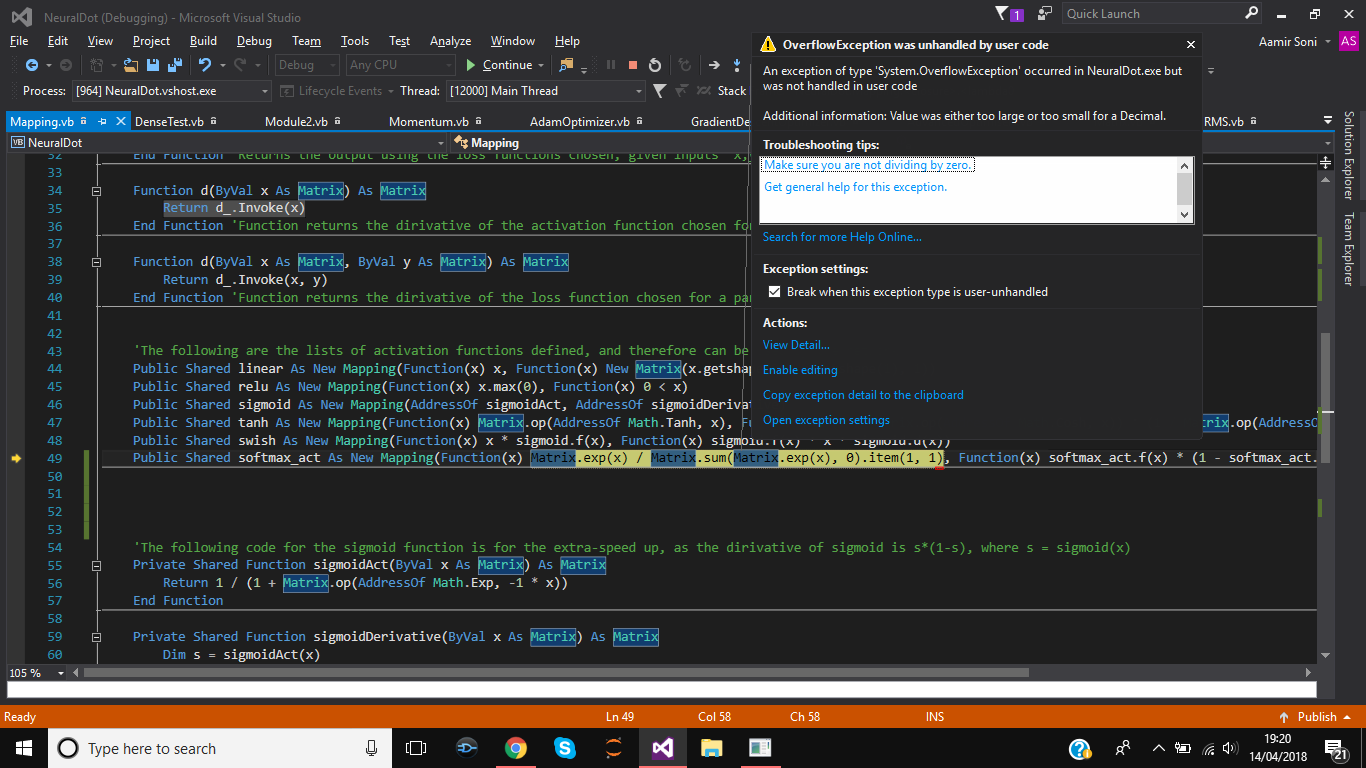
\includegraphics[width=10cm, height=5cm]{Testing/ConvTests/ExceptionHandlerConv1.png}
    \caption{Overflow Exception Handler}
    \label{TestNo3ResultsP2}
    
\end{figure}

This overflow exception was because the input was too large before the softmax function was applied. I solved this problem through using the fact that $ \frac{e^x_j}{\sum{e^x_i}} = \frac{e^{x_i - m}}{\sum{e^{(x_j - m)}}}$

Therefore, I have changed the line of code:

\begin{minted}[
frame=lines,
breaklines=true
]{vb.net}
    Public Shared softmax_act As New Mapping(Function(x) Matrix.exp(x) / Matrix.sum(Matrix.exp(x), 0).item(1, 1),Function(x) softmax_act.f(x) * (1 - softmax_act.f(x)))
\end{minted}
to 
\begin{minted}[
frame=lines,
breaklines=true
]{vb.net}
    Public Shared softmax_act As New Mapping(Function(x) Matrix.exp(x - x.max()) / Matrix.sum(Matrix.exp(x - x.max()), 0).item(1, 1), Function(x) softmax_act.f(x) * (1 - softmax_act.f(x)))
\end{minted}

This works because both the numerator and denominator of the fraction are being divided by $e^{x.max()}$, where $x.max()$ is the maximum element in the matrix, making all the values in the input matrix less than or equal to 1.
\\ \\
After changing this line, the nets worked perfectly fine. This shows that the convolutional networks are working as they should as the nets on average classified more than 90\% of the images correctly for each test, which means that the CNNs can now differentiate between images of numbers between 0 and 9. Finally, the time taken to train the CNNs was approximately 19 hours, which is mainly due to the reason that the convolution operation has time complexity $O(n^4)$.
